\documentclass[conference]{IEEEtran}
\IEEEoverridecommandlockouts
% The preceding line is only needed to identify funding in the first footnote. If that is unneeded, please comment it out.
\usepackage{cite}
\usepackage{amsmath,amssymb,amsfonts}
\usepackage{algorithmic}
\usepackage{graphicx}
\usepackage{textcomp}
\usepackage{xcolor}
\usepackage{color}
\usepackage{listings}
\usepackage{xparse}
\usepackage[spaces,hyphens]{url}
\usepackage{hyperref}

\def\BibTeX{{\rm B\kern-.05em{\sc i\kern-.025em b}\kern-.08em
    T\kern-.1667em\lower.7ex\hbox{E}\kern-.125emX}}
    
\NewDocumentCommand{\codeword}{v}{%
\texttt{\textcolor{blue}{#1}}%
}

\NewDocumentCommand{\tool}{v}{%
\texttt{\textcolor{gray}{#1}}%
}

\lstset{language=Bash,keywordstyle={\bfseries \color{blue}}}

\hypersetup{
    colorlinks=true,
    linkcolor=blue,
    filecolor=magenta,      
    urlcolor=cyan,
    pdftitle={Overleaf Example},
    pdfpagemode=FullScreen,
    }
    
\definecolor{dkgreen}{rgb}{0,0.6,0}
\definecolor{gray}{rgb}{0.5,0.5,0.5}
\definecolor{mauve}{rgb}{0.58,0,0.82}

\lstset{frame=tb,
  language=Bash,
  aboveskip=3mm,
  belowskip=3mm,
  showstringspaces=false,
  columns=flexible,
  basicstyle={\small\ttfamily},
  numbers=none,
  numberstyle=\tiny\color{gray},
  keywordstyle=\color{blue},
  commentstyle=\color{dkgreen},
  stringstyle=\color{mauve},
  breaklines=true,
  breakatwhitespace=true,
  tabsize=3
}

\begin{document}

\title{Mengenal OMNet++ dan Algoritma Dijkstra}

\author{\IEEEauthorblockN{Ricky}
	\IEEEauthorblockA{\textit{Teknik Komputer, Fakultas Teknologi Informasi} \\
		\textit{Institut Teknologi Batam}\\
		Batam, Indonesia \\
		1922022@student.iteba.ac.id}
	\and
	\IEEEauthorblockN{Muhamad Arie}
	\IEEEauthorblockA{\textit{Teknik Komputer, Fakultas Teknologi Informasi} \\
		\textit{Institut Teknologi Batam}\\
		Batam, Indonesia \\
		1922021@student.iteba.ac.id}
}
\maketitle

\begin{abstract}
	Omnet++ merupakan aplikasi dasar berbasis open source yang dituliskan menggunakan c++ untuk mendesain simulasi dan topologi jaringan. Disini kami akan mencoba mendesain sebuah topologi jaringan berisi 6 node dan dengan menggunakan algoritma Dijkstra, kita akan mencari jarak tersingkatnya.

\end{abstract}

\begin{IEEEkeywords}
	Simulation, Networking, Collision, Detection, Error, Correction
\end{IEEEkeywords}

\section{Pengenalan}
Tugas ini bertujuan untuk memberikan pengalamanan kepada mahasiswa untuk menggunakan OMNeT++. Tutorial ini memandu mahasiswa dalam membuat dan bekerja dengan contoh model simulasi,
dan menunjukkan beberapa fitur OMNeT ++ yang umum digunakan. Tutorial ini didasarkan pada
simulasi contoh Tictoc, yang dapat ditemukan di direktori samples/tictoc dari instalasi OMNeT++, sehingga mahasiswa dapat langsung mencoba contoh tersebut. Dan juga terdapat simulasi contoh Aloha yang dapat ditemukan di direktori samples/aloha. Versi OMNeT: 5.6.2. Lokasi file sumber:
tictoc1.ned, txc1.cc, omnetpp.ini

\section{Teori dan Tools}\label{teori-tool}
Simulasi jaringan adalah teknik di mana program perangkat lunak memodelkan perilaku jaringan dengan menghitung interaksi antara entitas jaringan yang berbeda (router, sakelar, node, titik akses, tautan, dll.). Kebanyakan simulator menggunakan simulasi kejadian diskrit - pemodelan sistem di mana variabel status berubah pada titik waktu tertentu. Perilaku jaringan dan berbagai aplikasi serta layanan yang didukungnya kemudian dapat diamati di lab uji; berbagai atribut \textit{environment} juga dapat dimodifikasi dengan cara yang terkontrol untuk menilai bagaimana jaringan / protokol akan berperilaku dalam kondisi yang berbeda.

Emulasi jaringan memungkinkan pengguna untuk memperkenalkan perangkat dan aplikasi nyata ke dalam jaringan uji (disimulasikan) yang mengubah aliran paket sedemikian rupa untuk meniru perilaku jaringan langsung. Lalu lintas langsung dapat melewati simulator dan dipengaruhi oleh objek dalam simulasi.

Metodologi tipikal adalah paket nyata(\textit{live packet}) dari aplikasi langsung dikirim ke server emulasi (tempat jaringan virtual disimulasikan). Paket sebenarnya \textbf{dimodulasi} menjadi paket simulasi. Paket simulasi didemodulasi menjadi paket nyata setelah mengalami efek kehilangan, kesalahan, penundaan, jitter, dll., Dengan demikian mentransfer efek jaringan ini ke paket nyata. Dengan demikian, seolah-olah paket nyata mengalir melalui jaringan nyata tetapi pada kenyataannya mengalir melalui jaringan yang disimulasikan. Emulasi digunakan secara luas dalam tahap desain untuk memvalidasi jaringan komunikasi sebelum penerapan.

Tools atau alat yang kami gunakan disini adalah \textit{fresh installed OMNet++} dengan samples bawaan yang sudah disediakan didalam folder instalasi.

\subsection{OMNeT++}
\textit{OMNeT++} adalah kerangka kerja simulasi jaringan peristiwa diskrit modular berorientasi objek. Memiliki arsitektur generik, sehingga dapat (dan telah) digunakan di berbagai domain masalah:

\begin{itemize}
	\item Permodelan jaringan komunikasi kabel dan nirkabel
	\item Permodelan protokol
	\item permodelan jaringan antrian
	\item Permodelan multiprosesor dan sistem perangkat keras terdistribusi lainnya
	\item Memvalidasi arsitektur perangkat keras
	\item Mengevaluasi aspek kinerja sistem perangkat lunak yang kompleks
	\item Secara umum, pemodelan dan simulasi sistem apa pun di mana pendekatan kejadian diskrit cocok, dan dapat dengan mudah dipetakan ke dalam entitas yang berkomunikasi dengan bertukar pesan.
\end{itemize}

\subsection{Algoritma Dijkstra}
Dijkstra adalah algoritma yang digunakan untuk mencari lintasan terpendek pada sebuah graf berarah. Contoh penerapan algoritma ini adalah lintasan terpendek yang menghubungkan antara dua kota ataupun titi berlainan tertentu. Algoritma Dijkstra bekerja dengan membuat jalur ke satu simpul optimal pada setiap langkah. Jadi pada langkah ke n, setidaknya ada n node yang sudah kita tahu jalur terpendek. Langkah - langkah algoritma Dijkstra dapat dilakukan dengan langkah - langkah berikut:
\begin{enumerate}
	\item Tentukan titik mana yang akan menjadi node awal, lalu beri bobot jarak pada node pertama ke node terdekat satu per satu, Dijkstra akan melakukan pengembangan pencarian dari satu titik ke titik lain dan ke titik selanjutnya tahap demi tahap.
	\item Beri nilai bobot (jarak) untuk setiap titik ke titik lainnya, lalu set nilai 0 pada node awal dan nilai tak hingga terhadap node lain (belum terisi) 2.
	\item Set semua node yang belum dilalui  dan set node awal sebagai “Node keberangkatan”.
	\item Dari node keberangkatan, pertimbangkan node tetangga yang belum dilalui dan hitung jaraknya dari titik keberangkatan. Jika jarak ini lebih kecil dari jarak sebelumnya (yang telah terekam sebelumnya) hapus data lama, simpan ulang data jarak dengan jarak yang baru.
	\item Saat kita selesai mempertimbangkan setiap jarak terhadap node tetangga, tandai node yang telah dilalui sebagai “Node dilewati”. Node yang dilewati tidak akan pernah di cek kembali, jarak yang disimpan adalah jarak terakhir dan yang paling minimal bobotnya.
	\item Set “Node belum dilewati” dengan jarak terkecil (dari node keberangkatan) sebagai “Node Keberangkatan” selanjutnya dan ulangi langkah e.
\end{enumerate}

\section{Pengerjaan}\label{pengerjaan}
Bagian ini akan membahas sedikit tentang cara kami mengerjakan, mulai dari metodologi hingga langkah-langkahnya:

\subsection{Metodologi}
Pada dasarnya tidak ada metode spesifik yang kami terapkan di \textit{Hands on} ini, kami hanya mengikuti \textit{official documentation} dari \textit{OMNet++}.

\subsection{Langkah Instalasi}
\begin{enumerate}
	\item Buka \href{https://omnetpp.org/}{\textit{official site OMNet++}}, lalu kunjungi bagian \href{https://omnetpp.org/intro}{\textit{Introduction}}. Baca sekilas pengenalan dengan \textit{OMNet++}.
	\item Download terlebih dahulu \textit{OMNet++} \href{https://omnetpp.org/download/}{disini}
	\item \textit{Extract zip} yang sudah didownload ke direktori yang diinginkan(nantinya akan menjadi direktori instalasi \textit{OMNet++}
	\item Buka direktori hasil \textit{extract} sebelumnya lalu \textit{double-click file} \codeword{mingwenv}, jalankan perintah \codeword{./configure} lalu tunggu hingga selesai. Setelah itu jalankan perintah \codeword{make} dan tunggu hingga selesai.
	\item Setelah itu kita dapat membuka IDE dengan mengetikkan perintah \codeword{omnetpp} di terminal \codeword{mingwenv}. Dan proses instalasi selesai
\end{enumerate}

untuk lebih lengkapnya tentang proses instalasi dapat mengikuti petunjuk \href{https://doc.omnetpp.org/omnetpp/InstallGuide.pdf}{disini}


\subsection{Flowchart}

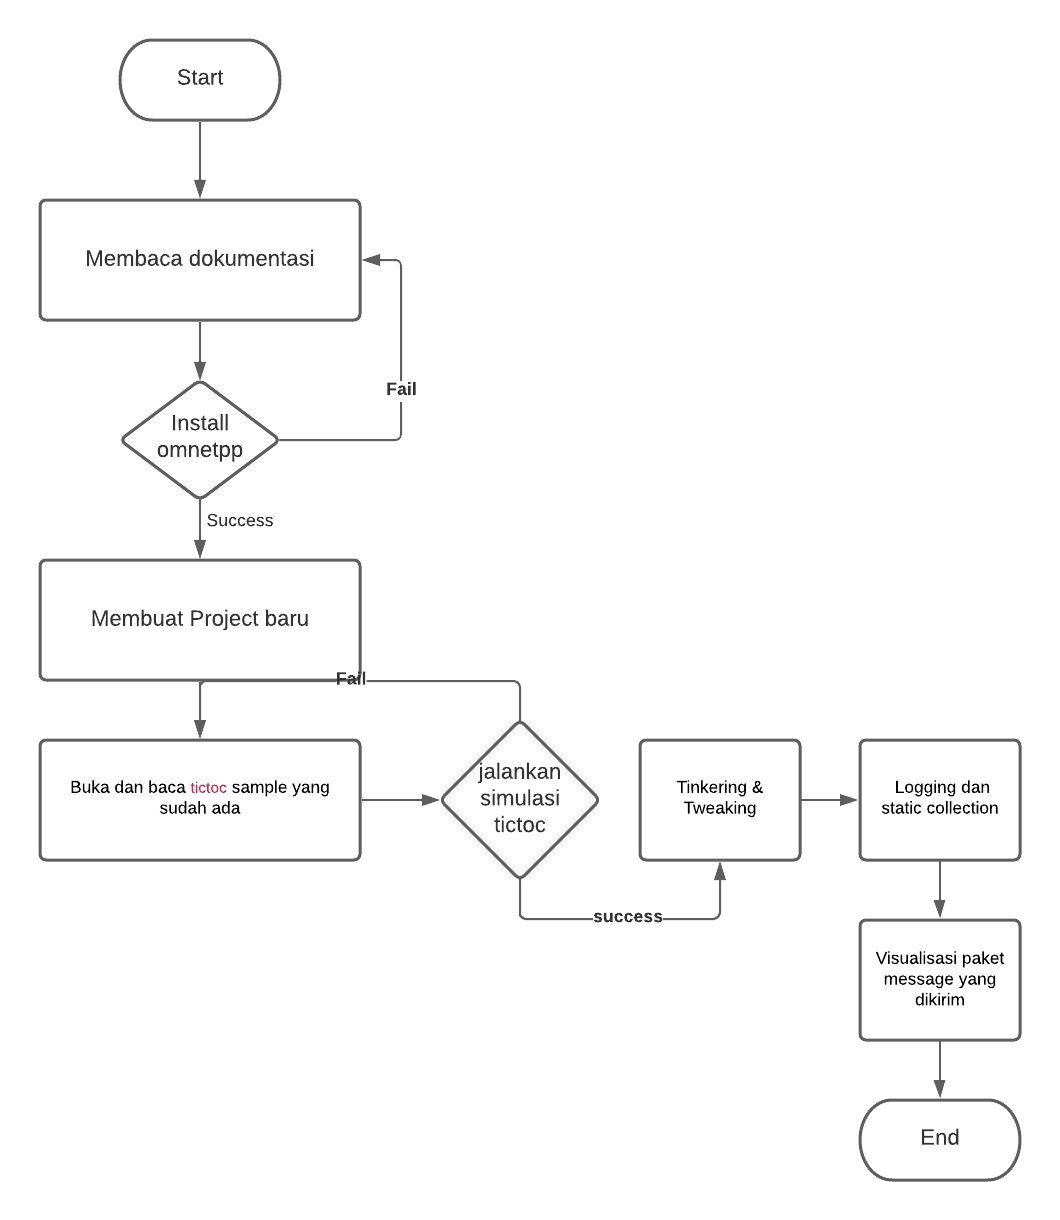
\includegraphics[scale=0.18]{images/flowchart.png}
\break

\section{Pembahasan}
Bagian ini akan menjelaskan secara singkat mengenai tiap bagian-bagian dari \textit{Tutorial Learn OMNeT++ with TicToc}. Namun kita tidak perlu mengikuti seluruh bagian yang dijelaskan pada halaman ini, seperti contohnya membuat \textit{sample} dan menambahkan \textit{NED file}. Dikarenakan saat kita menginstal sudah disediakan seluruh contohnya pada direktori \textit{samples/} beserta penjelasannya.

\subsection{Part 1: \href{https://docs.omnetpp.org/tutorials/tictoc/part1/}{Getting Started}}
Model pertama yang akan dikerjakan pada tutorial ini adalah model \textit{tic-toc}, dimana terdapat sebuah node yang saling mengirim dan menerima paket secara berulang. Ketika IDE sudah dibuka akan terlihat seperti gambar berikut,
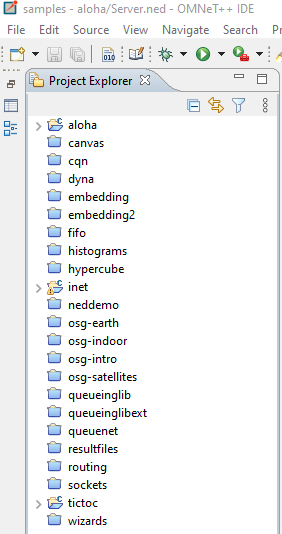
\includegraphics[scale=0.9]{images/samples-directory.png}


lalu buka \textit{tictoc} folder, didalamnya terdapat banyak sekali file. Pilih \codeword{tictoc1.ned}.

\subsection{Part 2: \href{https://docs.omnetpp.org/tutorials/tictoc/part2/}{Running the Simulation}}
Untuk menjalankan simulasinya, kita dapat menekan tombol \codeword{Run}\break
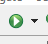
\includegraphics[scale=0.9]{images/run-button.png}

Akan terlihat sebuah \textit{console window} yang akan menjalankan proses \textit{Compiling}. Tunggu beberapa saat lalu akan muncul \textit{window} baru.\break 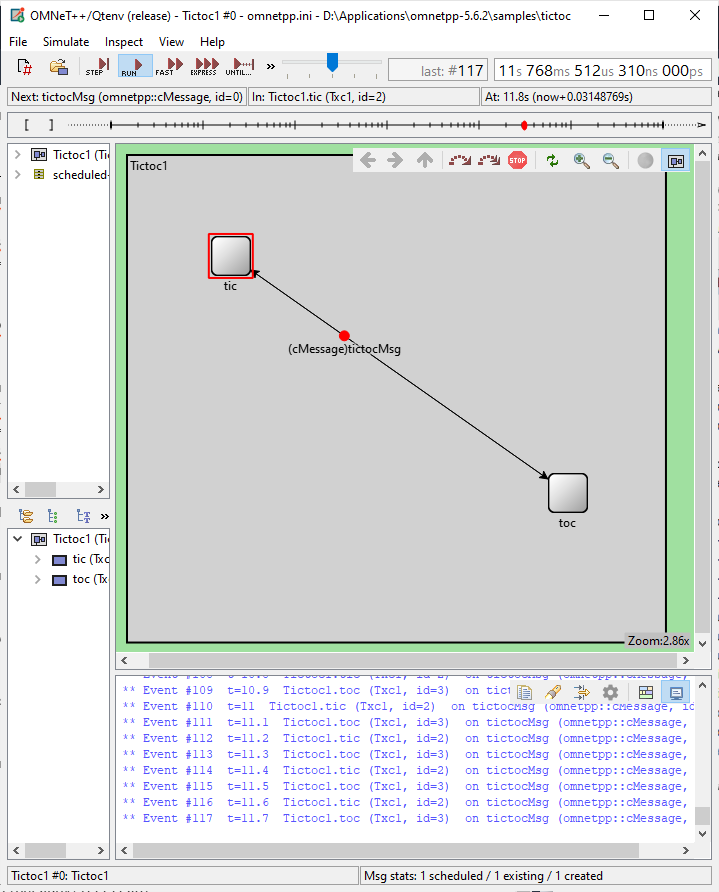
\includegraphics[scale=0.35]{images/simulation-window.png}

Dibagian ini juga kita dapat melakukan beberapa hal lainnya, seperti \textit{Debugging} dan \textit{Logging}, dapat juga memvisualisasikan menggunakan \textit{Sequence Chart}.

\subsection{Part 3: \href{https://docs.omnetpp.org/tutorials/tictoc/part3/}{Enhancing the 2-node TicToc}}
Pada bagian ini kita dapat meningkatkan \textit{2-node TicToc} menggunakan \textit{icon, logging, state variables, parameters, timers, etc}.

Untuk melihat contoh implementasi \textit{icon}, dapat membuka  dan menjalankan \textit{file} \codeword{tictoc2.ned}.\break

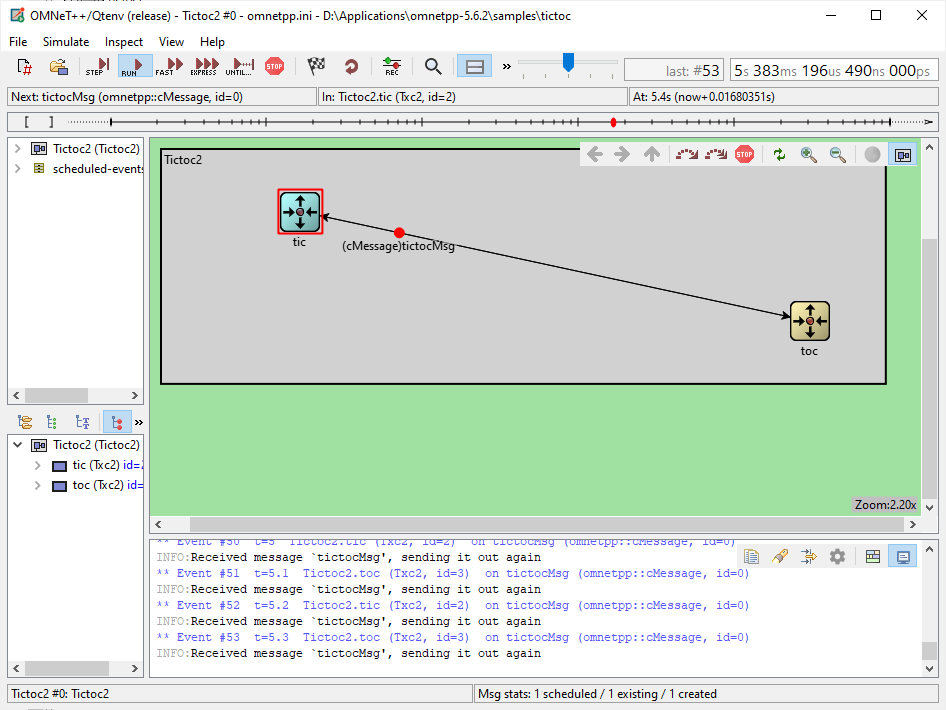
\includegraphics[scale=0.25]{images/tictoc2.ned.png}
\textit{Files:} \codeword{tictoc2.ned}, \codeword{txc2.cc}


untuk melihat contoh implementasi icon, silahkan buka \textit{file} \codeword{tictoc3.ned}. Jalankan simulasi dan klik kanan pada \textit{node}, klik menu \codeword{Open Component Log for 'tic'}. Akan muncul log seperti gambar berikut

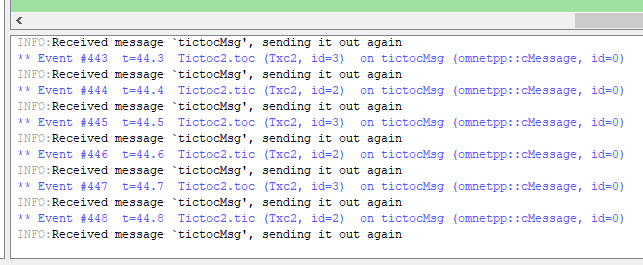
\includegraphics[scale=0.38]{images/tictoc3-log.ned.png}


selain itu terdapat beberapa \textit{file sample} yang dapat kita coba:
\begin{itemize}
	\item Parameters; \textit{Files: }\codeword{tictoc4.ned}, \codeword{txc4.cc}
	\item Timeout, cancelling timers; \textit{Files: }\codeword{tictoc8.ned}, \codeword{txc8.cc}
	\item etc
\end{itemize}

\subsection{Part 4: Turning it Into a Real Network}
Bagian ini akan menampilkan contoh implementasi lebih dari \textit{2 nodes}. Dapat membuka dan menjalankan simulasi \textit{file} \codeword{tictoc10.ned} . Kurang lebih akan terlihat seperti ini.
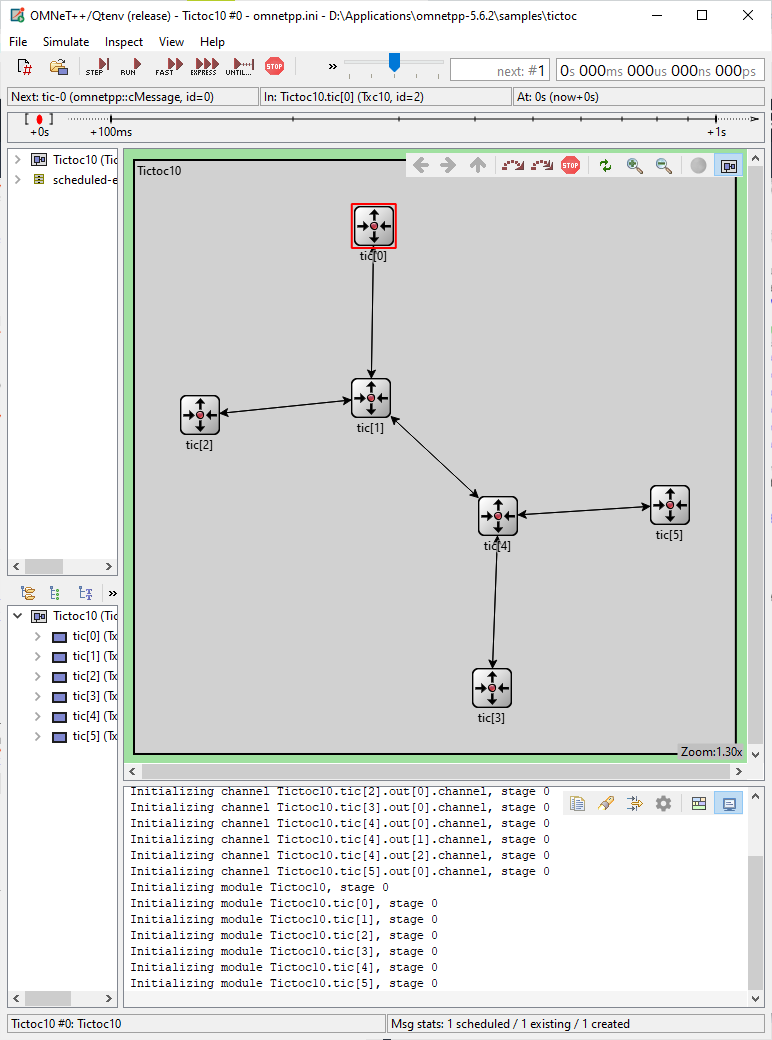
\includegraphics[scale=0.25]{images/tictoc10.ned.png}

\subsection{Part 5: Adding Statistics Collection}
Dari simulasi tersebut kita dapat mengumpulkan statistik data antar node juga. Seperti yang sudah diimplementasi di \codeword{txc14.cc}.

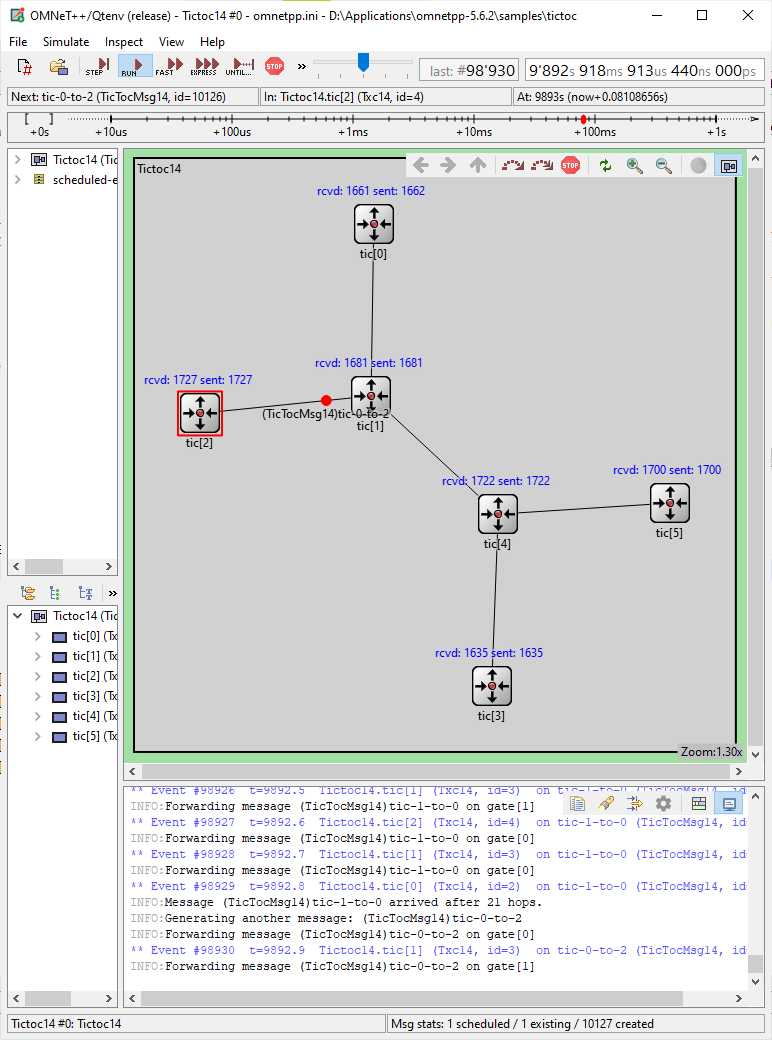
\includegraphics[scale=0.23]{images/tictoc14.ned.png}\break
\textit{Files:} \codeword{tictoc14.ned}, \codeword{tictoc14.msg}, \codeword{txc14.cc}

Kita dapat menampilkan Histogram data dengan cara sebagai berikut:
\begin{enumerate}
	\item Buka dan jalankan simulasi \textit{sample file} \codeword{tictoc15.ned} dengan mode \codeword{Fast} seperti gambar berikut\break
	      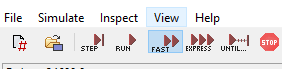
\includegraphics[scale=0.8]{images/fast-mode-button.png}

	\item Klik kanan pada \codeword{tic[1]}, lalu \codeword{Open Details for 'tic[1]'}\break
	      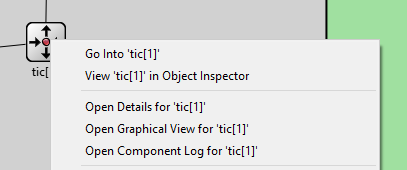
\includegraphics[scale=0.53]{images/tic[1].png}

	\item Setelah itu klik kanan lagi pada \codeword{hopCountStats}, lalu pilih \codeword{Open Graphical View for 'hopCountStats'}.\break
	      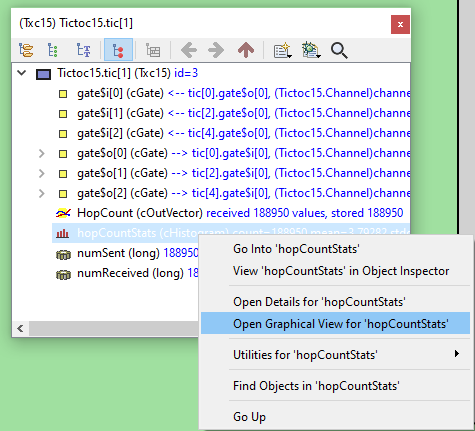
\includegraphics[scale=0.5]{images/tic[1]-histogram.png}. \break

	      Maka akan muncul Histogramnya seperti ini\break
	      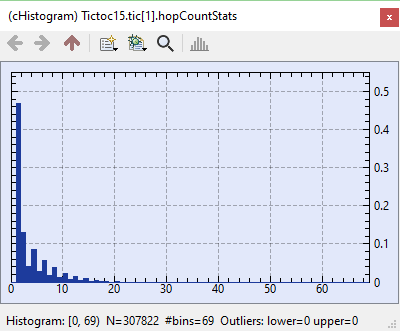
\includegraphics[scale=0.65]{images/tic[1]-histogram2.png}
\end{enumerate}

\subsection{Part 6: Visualizing the Results With the IDE}
Hasil dari \textit{static collection} dapat kita visualisasikan dalam berbagai model \textit{chart}. Berikut cara-caranya:
\begin{enumerate}
	\item Buka \textit{sample file} \codeword{tictoc/results/Tictoc15-#0.sca}
	\item Pada bagian bawah, klik \codeword{Browse Data}
	      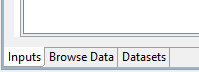
\includegraphics[scale=0.65]{images/browse-data-tab.png}
	      \newpage
	\item Lalu pilih \codeword{Vector} data
	      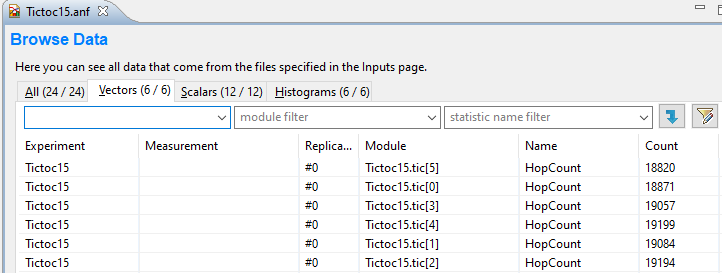
\includegraphics[scale=0.27]{images/vector-data.png}
	\item Lalu \textit{Select all}, klik kanan lalu \codeword{Plot}. Maka akan muncul data visualnya.
	      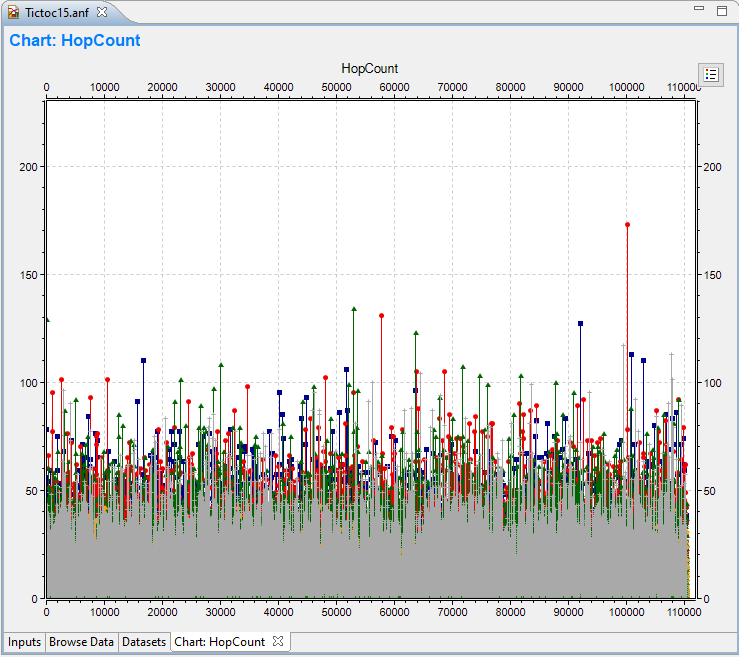
\includegraphics[scale=0.34]{images/plot-data.png}

	\item Pada \textit{background chart}, klik kanan \codeword{Properties}. Pada tab \codeword{Lines} kita dapat memilih \textit{Line type} dan \textit{Symbol type}. Pilih \codeword{Dots}
	\item Selanjutnya \textit{Display Legend} dengan cara, pilih menu \codeword{Legend} \textit{Display Legend}. \textit{Position above} dan \textit{Anchoring north}. Klik \textit{Ok}
\end{enumerate}

\subsection{Part 7: Parameter Studies}
Kita dapat menganalisis data yang sudah di \textit{record} dengan membuka \textit{file} yang berektensi \textit{.anf} , lalu pada tab \textit{Datasets} dapat dilihat dataset yang terdaftar.
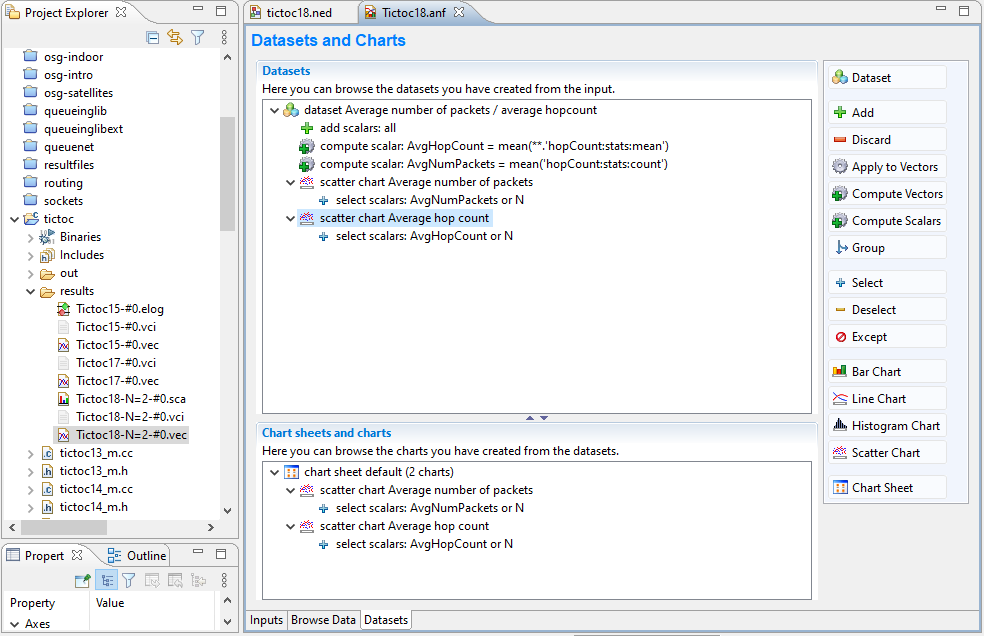
\includegraphics[scale=0.18]{images/tictoc18-analysis-file.png}

\section{Kesimpulan}
Kita dapat simpulkan bahwa simulasi jaringan berguna untuk meniru jaringan nyata sehingga kita dapat merencanakan rancangan, melakukan \textit{debugging}, dan juga analisis jaringan.

\bibliographystyle{./bibliography/IEEEtran}
\begin{thebibliography}{1}
	\bibitem{Installation Guide}\url{https://doc.omnetpp.org/omnetpp/InstallGuide.pdf}
	\bibitem{OMNet++ hands on Youtube}\url{https://youtu.be/u4T02tZuKrQ}
	\bibitem{OMNet++ TicToc tutorial}\url{https://docs.omnetpp.org/tutorials/tictoc}
	\bibitem{User Guide}\url{https://doc.omnetpp.org/omnetpp/UserGuide.pdf}
\end{thebibliography}

\end{document}
